\section{Task Formalization \& Modeling}

\begin{comment}
* Define the task
- Some math
- Several different application domains
    - augmentation
    - adversarial attack
    - extend data
    - counterfactual explanation
- Importance of where to change and how to change

* How to train
- Compute control tags
- Special tokens

* Use existing datasets
- Why each dataset 
- Data distribution [maybe appendix]

* Training hyperparameters

* Evaluations
- Filtering
- Diversity
\end{comment}
\subsection{Definitions, Applications, \& Properties}

\newcommand{\xset}{\mathbf{X}}
\newcommand{\yset}{\mathbf{Y}}
\newcommand{\gset}{\mathbf{G}}

\newcommand{\dset}{\mathcal{D}}
\newcommand{\xp}{\hat{x}}
\newcommand{\yp}{\hat{y}}

\begin{comment}
% Originally wanted a table to summarize 
\begin{table}
\small
\centering
\begin{tabular}{r c c}
\toprule

Application & \textbf{$y = \yp$} & $f(x)=f(\xp)$ \\ 
\midrule
Adversarial training 		& \cmark & \qmark \\
Data augmentation  			& \qmark & \qmark \\
Perturbation explanation 	& \qmark & \qmark \\
Adversarial training 		& \cmark & \qmark \\
\bottomrule
\end{tabular}

\caption{The datasets used for finetuning the GPT-2 perturbation model, and the \tagstr distributions.}
\label{table:gpt_train_stats}
\end{table}
\end{comment}



Suppose $\mathcal{X}$, $\mathcal{Y}$ denote the instance and label spaces of a dataset $\dset = \{ (x,y) | x \in \xset, y \in \yset \}\subset \mathcal{X} \times \mathcal{Y}$. We define a perturbation to be a mapping from an \emph{original} instance to a new, \emph{perturbed} one $\xp$.
The perturbation follow certain \emph{strategies} $s$ (e.g., negations~\cite{kaushik2019learning}, word substitution~\cite{li-etal-2020-bert-attack}, syntactical restructing~\cite{iyyer2018adversarial}).
The edited spans --- including a set of tokens removed from $x$ (denoted as $r(\xp)$) or newly added to $\xp$ ($a(\xp)$), and the affected parsing tree structures $t(\xp)$ --- are instantiations of the strategies.
For example, \swap{did}{didn't}, \swap{would never}{would} both instantiate for \ctrltag{negation}.
We aim to design a counterfactual generator $g$, such that for a given original instance $x$, we can gather multiple $\xp$ for the following applications, with desired properties.

\textbf{Applications.}
Perturbed examples have been used for training, evaluating, and explaining models decision boundaries.
Depending on whether they affect the model's groundtruth label, they can be categorized into \emph{adversarials} (\eg \citet{wu2019conditional} for training and \citet{jin2020bert} for evaluation) and \emph{counterfactuals} (\eg \citet{kaushik2019learning} for training and \citet{gardner2020contrast} for evaluation).
In the adversarial cases, the groundtruth label for $\xp$ are usually automatically determined and maintained, \ie $\yp = y$, whereas counterfactual ones require manual labeling~\cite{Khashabi2020MoreBF}, or a mapping between the perturbation templates and the resulting labels~\cite{li2020linguistically}.

\textbf{Properties.}
Desired perturbations are usually~\cite{morris2020textattack}:
(1) \emph{Minimally edited}, or $\xp$ is similar enough to $x$ to be considered as its variation; and 
(2) \emph{Grammatically correct and coherent}, or $\xp$ resembles $x$ enough that it has a high probability of being in the original $\xset$.
Additionally, augmentations usually prioritize (3) \emph{diversity} --- a group of $x$s are preturbed using various strategies, and various initiations under the same strategy, such that they provide different constraints on finetuning decision boundaries.
On the other hand, evaluations and explanations require more (4) \emph{controlled} perturbations for systematic and targeted inspections.
The diversity and the controllability are two competing factors, and prior work focusing on certain applications follow one of two extremes.
Those that thrive in diversity are either too uncontrolled (\eg text generation~\cite{iyyer2018adversarial}) or hard to scale (\eg manual rewrites~\cite{kaushik2019learning, gardner2020contrast}), whereas those that rely on templates or heuristic rules usually only cover limited linguistic patterns~\cite{li2020linguistically}.



\newcommand{\tagdefine}[1]{\emph{{\color{darkgray}#1} }}
\renewcommand{\arraystretch}{1.1}
\begin{table*}
\small
\centering
\begin{tabular}{p{0.11\linewidth} p{0.6\linewidth}  p{0.22\linewidth}}
\toprule
\textbf{\Tagstr} & \textbf{Definitions and Examples} & \textbf{Training datasets} \\ 
\midrule
\ctrltag{negation}
    & A dog is \add{not} embraced by the woman.
    & \cite{kaushik2019learning, gardner2020contrast}
\\ \midrule
\ctrltag{quantifier}
    & \swap{A dog is}{Three dogs are} embraced by the woman. 
    & \cite{gardner2020contrast}
\\ \midrule
\ctrltag{lexical}
    & \tagdefine{Changing just one word or noun chunks without breaking the POS tags.} \newline
      A dog is \swap{embraced}{attacked} by the woman.
    & \cite{sakaguchi2019winogrande}
\\ \midrule
\ctrltag{resemantic}
    & \tagdefine{To replace short phrases or clauses without affecting the parsing tree.}\newline
      A dog is \swap{embraced by the woman}{wrapped in a blanket}.
    & \cite{wieting2017paranmt}
\\ \midrule
\ctrltag{insert}
    & \tagdefine{To add constraints without affecting the parsing structure of other parts.} \newline
      A dog is embraced by the \add{little} woman.
    & \cite{wieting2017paranmt}
\\ \midrule
\ctrltag{delete}
    & \tagdefine{To remove constraints without affecting the parsing structure of other parts.} \newline
    A dog is embraced \remove{by the woman}.
    & \cite{wieting2017paranmt}
\\ \midrule
\ctrltag{restructure}
    & \tagdefine{To alter the dependency tree structure, \eg changing from passive to positive.} \newline
    A dog is \swap{embraced by}{hugging} the woman.
    & \cite{zhang2019paws, mccoy2019right}
\\ \midrule
\ctrltag{shuffle}
    & \tagdefine{To move (or swap) key phrases or entities around the sentence.} \newline
    A \swap{dog}{woman} is embraced by the \swap{woman}{dog}.
    & \cite{zhang2019paws, mccoy2019right}
\\
\bottomrule
\end{tabular}
\caption{A list of \tagstrs used for semantically driving the GPT-2 generation, their corresponding examples, and the training datasets that contains most of the corresponding patterns.
All the \add{perturbed examples} are generated by our finetuned model.}
%\wts{Change all the examples to be on an identical sentence, not all different cases. And consider further annotate the tags based on whether they just do semantic change or also syntactic change.}}
\label{table:ctrltag}
\end{table*}


\begin{figure}[t]
\centering
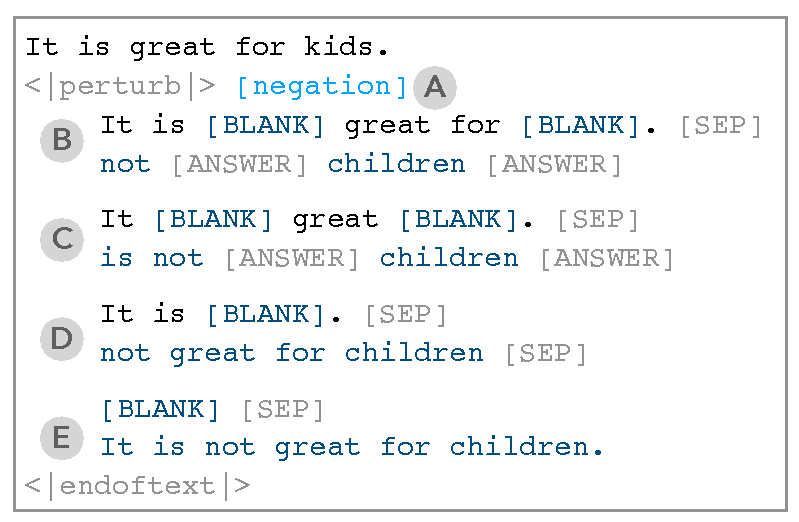
\includegraphics[width=1\columnwidth]{figures/blank}
\vspace{-15pt}
\caption{Given a pair of sentences $(x, \xp)$, we generate multiple training prompts with (A) a primary \tagstr, and various blanking strategies: (B) just the changed tokens, (C) the subtree of the changes, (D) the entire subphrase that contain all changes, and (E) the entire sentence.
We concatenate the information with special tokens like \perturbtoken.
}
\vspace{-10pt}
\label{fig:blank}
\end{figure}

\subsection{Perturbation as a NLG Task}

\paragraph{LM \& its prompts.}
In response to the objectives, we form the perturbation as a text generation task using language models (LM), which predict the continuing text given preceding prompts.
Here, instead of their common use case, \ie generating the remaining paragraphs, we use the original sentence $x$ as the prompt, and finetune off-the-shelf LMs to generate $\xp$: \exinline{$x$ \perturbtoken $\xp$ \stoptoken}.
We further modify the prompt structure as the following:

\emph{Enhance diversity with \tagstrs}.
LMs are naturally cover more strategies than small collections of templates or rewrite rules, but to further extend their perturbation diversity, we condition the generation on special tokens that denote the perturbation strategies (similar to \citet{raffel2019exploring, Dathathri2020Plug}).
We surveyed X papers related to text perturbations, and summarized 8 \tagstrs as in Table~\ref{table:ctrltag}.

We design these \tagstrs to cover commonly seen perturbations, and to maximize the syntactic differences between different groups, such that the controls are more explicit for the model to follow.
While it is also possible to use semantic-oriented \tagstrs (synonyms, antonyms, hyponyms, paraphrases), we found WordNet~\cite{miller1998wordnet} or sentence similarity based tagging are inaccurate, and the pattern was tricky to learn for the LM model.
Moreover, the \tagstrs distinguish the information change: the syntax-preserving ones add (\ctrltag{insert}), remove (\ctrltag{delete}), or change constraints, and the constraints vary from sparse (\ctrltag{resemantic} is more loose than \ctrltag{lexical}) to specific and finer-grained (\ctrltag{negation}, \ctrltag{quantifier}).
Remaining \ctrltag{shuffle} and \ctrltag{restructure}, on the other hand, focuses on syntactic understanding when we have high lexical overlap.

%\wts{Add some more explanation on the design rationale. It is a more syntactic style change, and we try to minimize the overlaps between words; But we leave out the semantic ones because they overlap too much. arguably lexical and resemantic are similar, but we separate them because editing distance and because too many prior work do lexical change that it deserves a separate category.}

\emph{Enable control with \BLANK}.
Besides boosting diversity, the \tagstrs also enable controls on \emph{how} to edit a sentence.
We further borrow the blank fill-in structure~\cite{donahue2020enabling} to control \emph{where} to edit, \ie targeted subphrases are replaced with special \BLANK tokens, and the actual content (``answers'' to blanks) are concatenated to the end. 

Note that to train a general-purpose perturbation model, we do not distinguish adversarials and counterfactuals, as they depend on the NLP tasks where the perturbations will be used --- Adding an adjective modifier ``blue'' may not affect the sentiment of a sentence, but may affect the labels in questions answering or natural language inferences.
Later in this paper, we mostly demonstrate applications related to manually labeled counterfactuals, but we believe the method can be easily generalized to the adversarial cases using some common filtering constraints (\eg sentence semantic similarity~\cite{morris2020textattack}).


\paragraph{Training data formation.}
\wts{This part is probably too long.}
While we do not have a single NLP dataset designed for strategy-driven perturbation, multiple existing datasets can each express a subset of the perturbation strategy patterns.
We survey multiple datasets with paired sentences, and combined six of them into a training set that cover all \tagstrs.
We additionally crawled some sentence pairs from non-paired datasets like SQuAD~\cite{rajpurkar-etal-2016-squad} to boost some specific patterns and increase lexical diversity. 
We list some of the representative datasets for each \tagstr in Table~\ref{table:ctrltag}, and describe them in more details in \S\ref{appendix:train_data}.

Given a pair, we use the two sentences interchangeably as $x$ and $\xp$ to learn the perturbations both ways.
We compute its primary \tagstr based on linguistic features like part-of-speech tagging or dependency trees, and blank out the changed subphrases in $\xp$.
For example, \ctrltag{negation} occurs when we observe changes on negation modifiers or specific words like ``supposedly'', and \ctrltag{shuffle} occurs when we have overlaps between tokens deleted and added.
When multiple changes occur, we label it with the primary \tagstr, which most significantly change the semantic meaning on the corresponding subphrase 
In Figure~\ref{fig:blank}, we use the tag \ctrltag{negation}, as \swap{good}{not good} is more significant than \swap{movie}{book}.
If we cannot identify the \tagstr for a pair or if the editing distance is too large, we denote it with \ctrltag{[global]} and use them as negative samples.
Importantly, to allow flexible blanking at the generation time, instead of merely blanking the edited spans, we also extend the blank to cover their associated parsing structures, etc.
As a result, we form up to four unique training prompts given one $(x, \xp)$ pair (Figure~\ref{fig:blank}).

%max_log_prob_diff

We put \tagstrs before $\xp$ because we would like to prioritize \emph{how} over \emph{where}, such that when given a \tagstr, the model can determine the appropriate changing places, and generate the blanked prompt on its own. 
However, in cases where it is more essential to inspect particular subphrases, it is possible to reverse the order, so we can provide the blanked prompts, and let the model figure out the \emph{how}.
%It is also possible to swap the order of the blanked $\xp$ and the \tagstrs. 

With the interchangeable orders and the blanks, we generate 657,144 training prompts from 191,415 sentence pairs.
We use the data to finetune an off-the-shelf GPT-2 model (from \citet{Wolf2019HuggingFacesTS}), but any LM can potentially be used.
\wts{Add the training hyperparameters; And maybe eventually move them to appendix.}
We finetuned the model for 3 epochs, with an initial learning rate 5e-5, a batch size of 16 and a sequence length of 120.

\paragraph{Filtering on the generations.}
The infilling structure does not always generate \emph{valid} sentences, and therefore require additional filtering.
Inspired by the language model constraints in \citet{morris2020textattack}, we score both $x$ and $\xp$ using un-finetuned GPT-2, and invalidate all $\xp$ whose log-probability (either on the full sentence or on the perturbed chunks) decreases more than $k=10$ points compared to $x$ (though their other constraints may also be useful.)


%pr["pr_sent"]<=10 and pr["pr_phrase"] <=10
%Perplexity is instantiating; Language modeling as an approximation because it measures real world distribution.

%\& Ablation Studies
\subsection{Intrinsic Evaluations}
% random no-pair models. 1142508
We verify the impact of the filtering and the \tagstrs through human evaluations.
\paragraph{Validity.}
One of the coauthors manually labeled the validity of 600 augmentations generated on 120 instances from three datasets: \dsst~\cite{socher2013recursive}, \dnli~\cite{bowman-etal-2015-large}, and \dqqp~\cite{wang2018glue}.
The validity rate among all the generated instances were $61.5\%$, which increased to $78.3\%$ after the filtering. 
As part of the data labeling task in \S\ref{sec:app_label}, we also asked crowdworkers to label whether a perturbed sentence is valid (\emph{``whether the sentence is grammatically correct and semantically meaningful, likely written by a native English speaker''}), and they arrived at similar validation rates ($75.0\%$ for \dsst, $70.0\%$ for \dqqp, and $81.7\%$ for \dnli).
%If no filter at all, the instances you see will only have 60% valid stuff (we care more about precision, every invalid counterfactual shown to a human is wasted time):
\wts{Maybe no need for the instruction; It's in appendix.}


\paragraph{Controllability.}
We observed that model does not always follow it for three reasons:
(1) The dual manipulation from \tagstrs and \BLANK sometimes conflict, \eg \exinline{a dog is embraced by a [BLANK]} would not respond to \ctrltag{negation}.
(2) $x$ does not have the corresponding pattern. \ctrltag{shuffle} is not applicable when the sentence does not have more than one adjective or NOUN (\eg \exinline{the movie is good}).
(3) The pattern-to-perturb is very prominent that it dominates the generation probability. 
For example, the model tends to perturb the quantifier ``two'' in \exinline{two dogs are running}, regardless of the tag.

That said, we still verify that \tagstrs successfully impact the generation.
We selected X sentences that can potentially allow all the defined changes, and generated perturbations with all \tagstr inputs through beam search, and re-compute the \tagstr on each output.
We deem the control successful if at least one of the output \tagstr matches the input in the top 3 returns.
The succesful rate was X, ranging from X (tag1) to X (tag2.)
\wts{TODO}
With an ablation study training models without \tagstr or without \BLANK, we ...
\wts{tag diversity, bleu}

%\paragraph{Diversity.}






